\section{簡介}
接續前一章所提到,我們需要使用一個過濾器,從檢索的回傳值中挑選出最可能含有答案的文本。困難的點在,這並非僅僅是找尋文本中是否包含有查詢詞,因為這在檢索時已經使用過了。更深入的是,我們需要能夠判別語意是否能夠回答到查詢詞。故在此若僅只是使用詞頻(Term Frequency,tf)- 逆向檔案頻率(Inverse Document Frequency,idf),對於要選擇出是否包含著答案的文本並不容易。對此,我們使用了相同的模型來解決這件事情,差別僅僅是把編碼器編碼後的結果,通過一層分類器來判別文本是否有包含查詢詞,最後預測值大於 0.5 則判定為相關,如圖( \ref{fig:dmn_classifier} )

\section{基本實驗配置}
%TODO tf-idf baseline
\subsection{卷積類神經網路(Convolutional Nueral Network)}
卷積神經網路 \cite{sharif2014cnn}(Convolutional Nueral Network, CNN),為深層類神經網路的一種變形,特色是局部感知以及參數共享。主要組成為卷積層(Convolutional Layers)和合計層(Pooling Layer)。其對於二維的輸入資料有更好的理解,如圖像,甚至在自然語言領域裡也被證實比遞迴式類神經網路有更好的結果,且因為可平行處理,能夠獲得更快速的訓練與測試。以下將大略介紹兩個組成。
\begin{itemize}
    \itemsep - 2pt
    \item 卷積層\\
        卷積層主要由一系列的卷積單元構成,又稱為核心(Kernel)或過濾器(Filter),每個核心含有一些可訓練的參數,與深層類神經網路的概念一樣。每層有很多個核心,每個核心專門負責學習一些特徵,若是該輸入的部分含有此特徵,則會被激發。整個卷積類神經網路可以有很多層,而越低層的可以學習到較具體的特徵;越高層則能學到較抽象的特徵。
    \item 合計層 \\
        合計層為一縮減採樣(Down-Sampling),在通過卷積層後,特徵會過多,容易過度貼合,學習也不易,因此大多會計算某區域特徵的平均值或最大值,以便簡化特徵數量。
\end{itemize}

在本章節,我們提出兩個基準實驗模型,如圖 \ref{fig:gru_classifier} 、\ref{fig:cnn_classifier} ,差別在文本讀取的方式,是使用遞迴式類神經網路抑或是卷積類神經網路。
\begin{figure}[h]
    \centering
    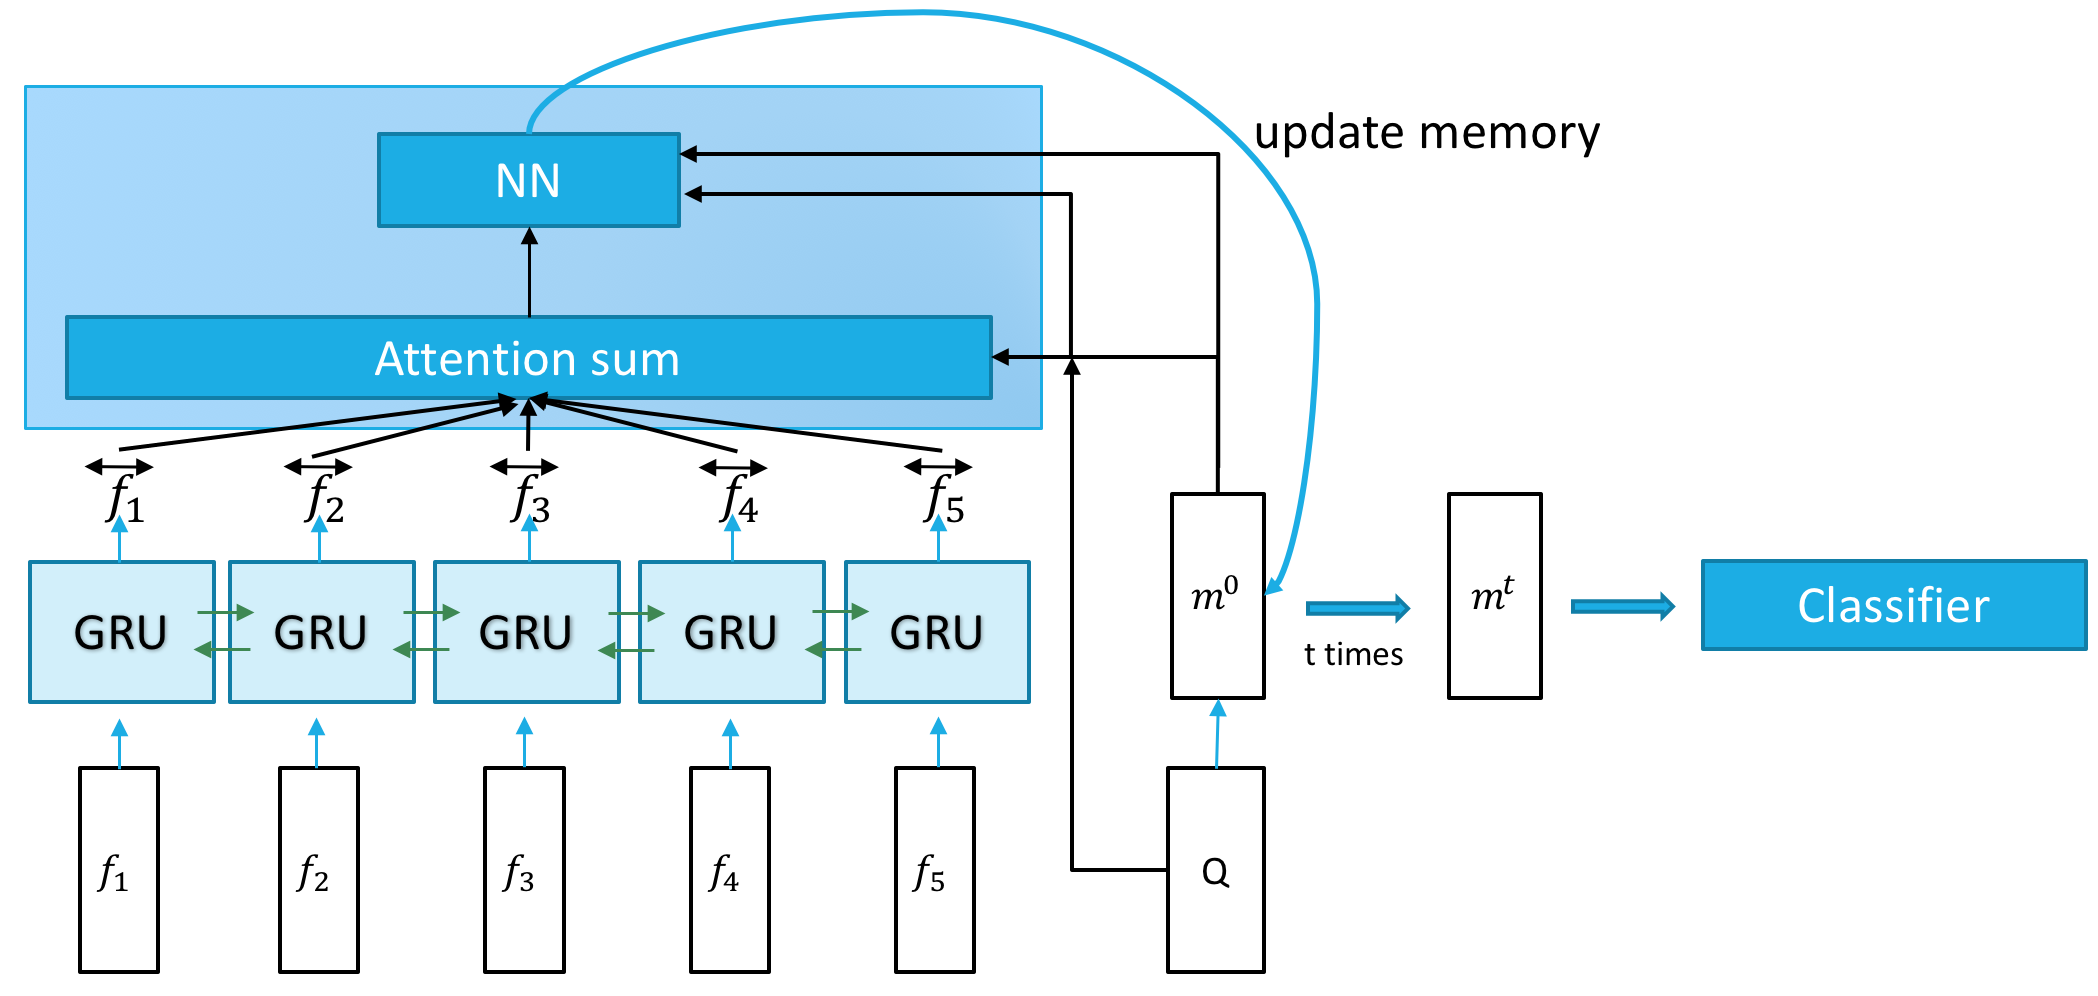
\includegraphics[scale=0.5]{images/chap4_dmn.png}
    \caption{分類器模型}
    \label{fig:dmn_classifier}
\end{figure}

\begin{figure}
    \centering
    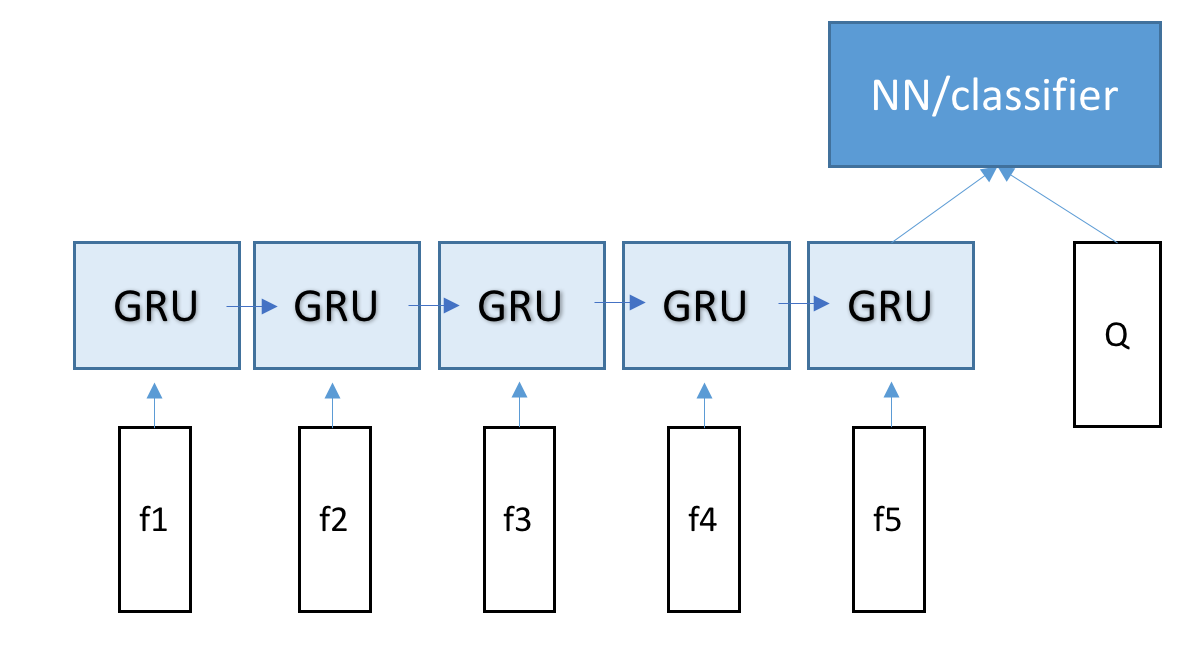
\includegraphics[scale=0.5]{images/chap4_gru.png}
    \caption{遞迴式分類器}
    \label{fig:gru_classifier}
\end{figure}

\begin{figure}
    \centering
    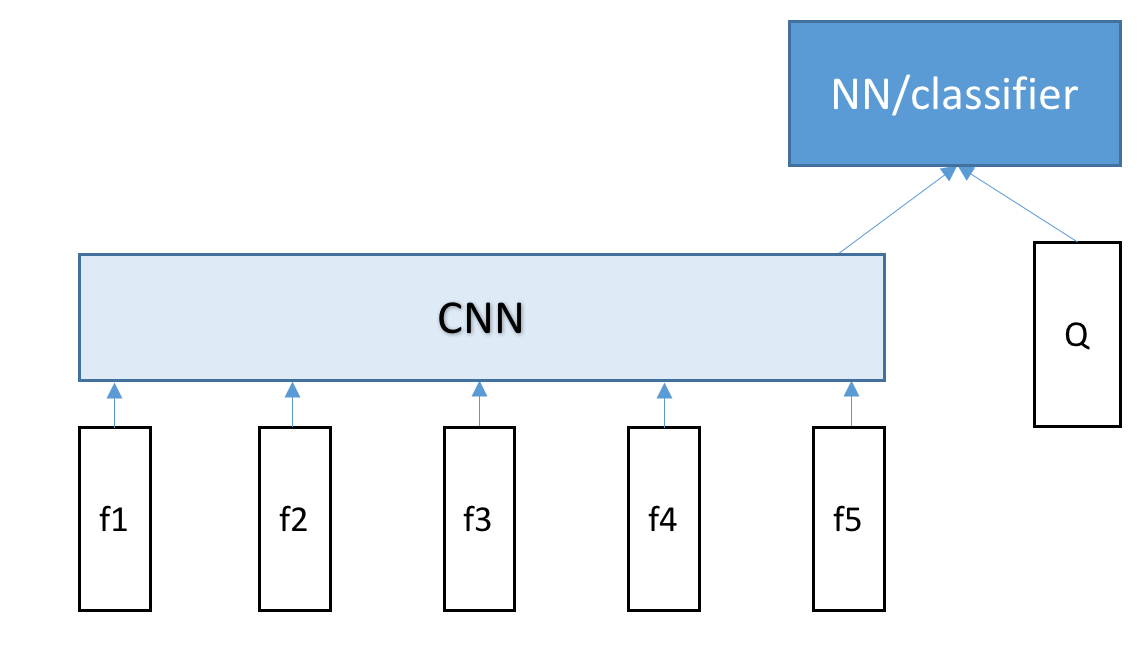
\includegraphics[scale=0.5]{images/chap4_cnn.png}
    \caption{卷積分類器}
    \label{fig:cnn_classifier}
\end{figure}

\section{實驗結果與討論}
%TODO MAP
如我們一開始所提到,TF-IDF 要能成功選出相關文本並不容易,實驗結果顯示其 F 度量(F-Measure)僅只有 0.22 。然而對於在此章節,模型表現並不如我們所預期,雖然在訓練集中準確率可達 0.95 左右,且 F 度量(F-measure)分數也有 0.80 ,但在測試集中,只有約莫 0.8 的準確率,F 度量亦只有 0.19 。

雖然在一開始我們訓練時是依據分類器所給機率是否在 0.5 以上來決定是否相關,但為了避免測試下來都與問句想要的答案無關,或者是過多與其相關,我們在此處選擇模型預測之最高分數的文章當作相關文章,其餘當作不相關進行測試,表 \ref{table:classifier} 為其結果。由實驗結果可明顯知道,結果並不如我們所預期,而且雖然專注式模型的 F 度量比其餘兩者都好,但在 ROUGE 的分數卻比較差,推測可能僅是些微的誤差,並不能代表真實成果的高低。雖然說這個結果不好,但也間接證明了第三章的模型,能回答出正確的答案並非意外,而是真的能從文章之中選取出答案。
%TODO
\begin{table}[ht]
    \caption{分類器比較} 
    \label{table:classifier}
    \centering
    \begin{tabular}{|l|l|}
        \hline
        分類器種類 & ROUGE\\
        \hline
        RNN & 16.01\%\\%Mazu\\
        \hline
        CNN & 14.88\%\\%Athena\\
        \hline
        專注式記憶模型 & 15.96\%\\%Venus\\
        \hline
    \end{tabular}
\end{table}
\section{本章總結}
本章節雖未有像第三章之表現,但實際上 F 度量並沒有非常差,且在訓練資料上已經過度貼合,或許在稍加改進模型就能夠有好的結果。而這章節也另類的顯示出有相對應的文章,即有辦法回答出相似的結果,而非沒有靠文章才回答問題。
